\section{The Perceptron}
\label{sec:perceptron}
The perceptron\cite{McCulloch1943115} is a simple mathematical model of the biological neuron. It accepts $n$ input values $x_1, \ldots, x_n$ and computes a corresponding output by computing the weighted sum
\begin{equation}\label{eq:perceptron1}
	\sum_{i=1}^{n} w_ix_i,
\end{equation}
where the weights $w_i$ are the parameters of the model.
By representing the input values as a vector $\bm{x}$ and the weights as a vector $\bm{w}$, we can rewrite \eqref{eq:perceptron1} as $\bm{w}^\top\bm{x}$. Fig. \ref{fig:perceptron} illustrates the perceptron.

\begin{figure}
	\begin{center}
		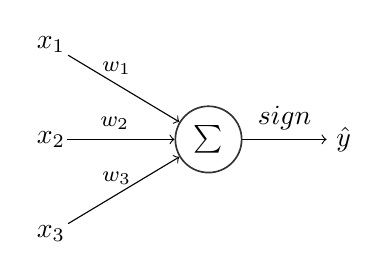
\begin{tikzpicture}
	\tikzstyle{neuron} = [circle,draw=black!80,semithick,minimum size=20pt]
	% input layer
	\foreach \i in {1,...,3}
		\node (input\i) at (0, -\i*1.2) {$x_\i$};
	% perceptron
	\node[neuron] (perceptron) at (2, -2*1.2) {$\sum$};
	% connections
	\foreach \i in {1,...,3}
		\draw[->, shorten <= -.1cm] (input\i) -- node[pos=.4,above]{\footnotesize{$w_\i$}} (perceptron);
	% output
	\draw[->] (perceptron) -- node[above]{$\text{sign}$}(3.5, -2*1.2) node[right]{$\hat{y}$};
\end{tikzpicture}
	\end{center}
	\caption{An illustration of the perceptron model. In this example, the perceptron accepts three inputs $x_1, x_2, x_3$ and computes the weighted sum $w_1x_1 + w_2x_2 + w_3x_3.$}
	\label{fig:perceptron}
\end{figure}

One usecase of the perceptron are binary classification problems. Given a set of $m$ training examples $\mathbb{X} = \{\bm{x}^{(1)}, \ldots, \bm{x}^{(m)}\}$ and their corresponding binary labels $\mathbb{Y}$, we want to predict whether a given vector $\bm{x}$ is more likely to have the label $y = 1$ or the label $y = -1$.

For example, our vectors $\bm{x}^{(i)}$ might describe features of an email using a \emph{bag-of-words} representation. That is, we specify a fixed vocabulary of words and the $j$th entry in the vector specifies how often the $j$th word of the vocabulary occurs in that particular document. The corresponding label $y^{(i)} = 1$ then might signify that the email was a legitimate email, whereas a value of $y^{(i)} = -1$ might label the email as spam.

Prediction with the perceptron model is simple: We predict a value $\hat{y}$ depending on the sign of the weighted sum:
\begin{equation}
\hat{y} = \begin{cases} 1 & \text{if }\bm{w}^{\top}\bm{x} \geq 0,
					  \\-1 & \text{if }\bm{w}^{\top}\bm{x} < 0.
		  \end{cases}
\end{equation}

The weights are randomly initialized and the model thus makes arbitrary predictions in the beginning. In the process of \emph{training} the perceptron, we iteratively adjust the weights so that the predictions on the ovserved training data $\mathbb{X}$ improve.

One way to train the model is the perceptron learning algorithm proposed by \cite{Rosenblatt1958386}. The intuition behind the algorithm is that we step through the training data and only update $\bm{w}$ if the label that the model predicts is different from the actual observed label. However, if the model predicts a positive label and the actual label is negative, we adjust all weights corresponding to the training example a little in the negative direction, and we adjust the weights in the positive direction in the opposite case. Details can be found in ??.

As we have seen, the perceptron is a rather simple model and it is thus no surprise that its performance is rather poor. In particular, it can be shown that the perceptron can only learn to classify linearly separable data [??]. For example, no combination of weights can successfully solve the \textsc{xor} problem \ldots.

More sophisticated models needed which eventually led to the development of the neural network.